\documentclass[a4paper]{article}

\usepackage[english]{babel}
\usepackage{amsmath}
\usepackage{graphicx}
%\usepackage{algorithm}
%\usepackage{algorithmic}
%\usepackage{algpseudocode}
\usepackage{url}


\title{Omega3P+PUMI Progress Report}

\author{Cameron W. Smith, Gerrett Diamond}

\date{\today}

\begin{document}
\maketitle
\section{Intro}

Unstructured mesh methods, like finite elements and finite volumes, support the 
effective analysis of complex physical behaviors modeled by partial differential
equations over general three-dimensional domains.
The most reliable and efficient methods apply adaptive procedures with
a-posteriori error estimators that indicate where and how the mesh is to be
modified.
Although adaptive meshes can have two to three orders of magnitude fewer
elements than a more uniform mesh for the same level of accuracy, there are many
complex simulations where the meshes required are so large that they can only be
solved on massively parallel systems.

Parallel simulations on massively parallel systems are most effective when data
movement is minimized.
Data movement costs increase with the depth of the memory hierarchy; a design
trade-off for increased capacity.
For example, the highest level on-node storage in the IBM BlueGene/Q A2
processor~\cite{haring2012ibm} is the per-core 16KiB L1 cache (excluding
registers) and has a peak bandwidth of 819 GiB/s.
The lowest level on-node storage, 16GiB of DDR3 main memory, provides a million
times more capacity at the cost of 19 times less bandwidth,
43GiB/s~\cite{lo2014roofline}.
One level further down the hierarchy is the parallel filesystem
~\footnote{We assume, for the sake of simplicity, that the main memory of other nodes is not
available.
In practice, most applications do not not use all the on-node memory and some
checkpoint-restart methods take advantage of this for increased performance
~\cite{rma-fault-tolerance-2014,isaila2014making,compression-cr-2012}.
}.
At this level the bandwidth and capacity relationship is less clear as the
filesystem is a shared resource.
Table~\ref{tbl:systems} lists the per-node peak main memory and filesystem
bandwidth across four generations of Argonne National Laboratory leadership
class systems: BlueGene/L~\cite{yu2006high,adiga2002overview}, Intrepid
BlueGene/P~\cite{lang2009performance,alam2008early}, Mira
BlueGene/Q~\cite{haring2012ibm,bui2014scalable}, and 2018's
Aurora~\cite{aurorafacts}.
Based on these peak values the bandwidth gap between main memory and the
filesystem is at least three orders of magnitude.
Software must leverage the cache and main memory bandwidth performance advantage
during as many operations as possible to maximize performance.

\begin{table}[h]
\centering
\caption{Per-node main memory and filesystem peak bandwidth over four
  generations of Argonne National Laboratory systems.
  The values in parentheses indicate the increase relative to
  the previous generation system.}
\label{tbl:systems}
\begin{tabular}{l|cc}
        & Memory BW & Filesystem BW \\
        & (GiB/s)    & (GiB/s)    \\
 \hline
 BG/L   & 5.6       & 0.0039         \\
 BG/P   & 14 (2.4x) & 0.0014 (0.36x)   \\
 BG/Q   & 43 (3.1x) & 0.0049 (3.5x) \\
 Aurora & 600 (14x) & 0.020 (4.1x)
\end{tabular}
\end{table}

We begin the report by discussing techniques for in-memory software interactions
that avoid file I/O.
Section~\ref{sec:inmem} concludes with a discussion of the Omega3P-PUMI
in-memory integration.
Next, Section~\ref{sec:parma} discusses the integration of the PUMI tools
for static and dynamic load balancing for Omega3P.
Section~\ref{sec:software} briefly lists ACE3P software improvements.
Section~\ref{sec:results} concludes the report with closing remarks and next
steps.

\section{In-memory Integration}\label{sec:inmem}

Approaches for high performing and scalable component interactions avoid
file-based I/O through in-memory data streams and component functional
interfaces.

The ADIOS tools provide an alternative mechanism for the in-memory coupling of
executables~\cite{bennett2012combining,zhang2012enabling}; our work here focuses
on the interaction of libraries operating within the same process.
Components that support a common file format can use our data stream approach
with minimal software changes to exchange data via memory buffers instead of files.
This approach is also a logical choice for legacy analysis codes that do not
provide functional interfaces to access or create their input and output data
structures.

Components with functional interfaces that encapsulate creation, deletion, and
access to underlying data structures support in-memory interactions.
The level of interface granularity selected for defining interactions has a
proportional impact on flexibility and development costs.
At a very fine level a developer may implement all mesh entity query functions such
that components can share the same mesh structure; trading increased development
costs for lower runtime memory usage.
An excellent example of this is the use of octree structures in the
development of parallel adaptive analyses~\cite{BursteddeWilcoxGhattas11}.
At a coarser level a developer may simply create another mesh
representation through use of interfaces encapsulating mesh construction;
trading higher runtime memory usage for lower development costs.
For example, an existing solver component can embed low level
calls to mesh-entity iterators~\cite{Ollivier10}.
Although this method will allow for in-memory integration, it suffers from the
same disadvantages as a tightly coupled approach in that a significant amount of
time and effort will be required for code modification and verification.
A generalization of this coarser level approach defines common sets of
interfaces through which all components interact.
For example, in the rotorcraft aerodynamics community the HELIOS platform
provides a set of analysis, meshing, adaptation, and load balancing components
via the Python-based Software Integration Framework~\cite{sankaran2010application}.

Our implementation of in-memory integration for PUMI and Omega3p uses
mesh query and construction APIs for mesh and field conversion combined with
fine-level APIs for querying higher-order geometric data for element
integrals. 
%technical details
Our conversion begins with a version of Omega3P's netcdf file reader that is altered 
to read the mesh data into PUMI data structures instead of Omega3P's Distmesh. With 
the PUMI mesh we are able to perform partitioning and load balancing as well as adaptation 
while only storing the PUMI mesh. After we have a finalized PUMI mesh a second 
overloaded version of Omega3P's file reader is used to convert the PUMI mesh to 
Omega3P's DistMesh. This is done by using the data from the in-memory PUMI mesh as the 
input instead of the netcdf file. After the conversion to DistMesh, we store both the 
PUMI Mesh and the Omega3P DistMesh for the duration of the finite element setup and 
computations. The reading and converting of the mesh data together take less than 15\% 
of the total runtime and have a similar cost to the netcdf read since the conversion 
from PUMI to Distmesh is much faster than both the original file reading to Distmesh 
and the new file reading to PUMI. 
%Memory discussion (needs revisions?)
The dual mesh approach offers code simplicity and 
ease of access for both structures at the cost of increased peak memory usage. 
Figure \ref{fig:memusage} shows the peak memory usage over the entire program for both
the original Omega3P code and with the PUMI mesh. The increase in peak memory when 
storing the PUMI mesh is 2\% at 64 cores and 8\% at 128 cores. At 32 cores the 
peak memory usage is less for the run with the PUMI mesh likely due to a better 
partition of the mesh. 
%Could probably use some smoothing to the next point
Mesh conversion alone is not sufficient to integrate over elements near the
geometric boundary.
We support these integrals by implementing Omega3P geometric queries with PUMI
APIs that can interrogate parametric model information provided by CAD
kernels.
CWS - SAY MORE!!!!

\section{Load Balancing}\label{sec:parma}

The Omega3P solving step relies on both on part mesh entities as well as a layer of 
ghosted elements along each part boundary. Omega3P's ghosting uses vertex adjacency such
that every element that shares a vertex with a part boundary will be ghosted to each part that shares that boundary. This can be seen in Figure \ref{fig:ghost3} that shows an 
example of a mesh with a layer of ghosting. In order to reach maximum efficiency
for Omega3P, partitioning must target minimizing the sum of the 
ghosted and on-part elements as well as the mesh entities holding degrees-of-freedom.

\begin{figure}[ht]
\centering
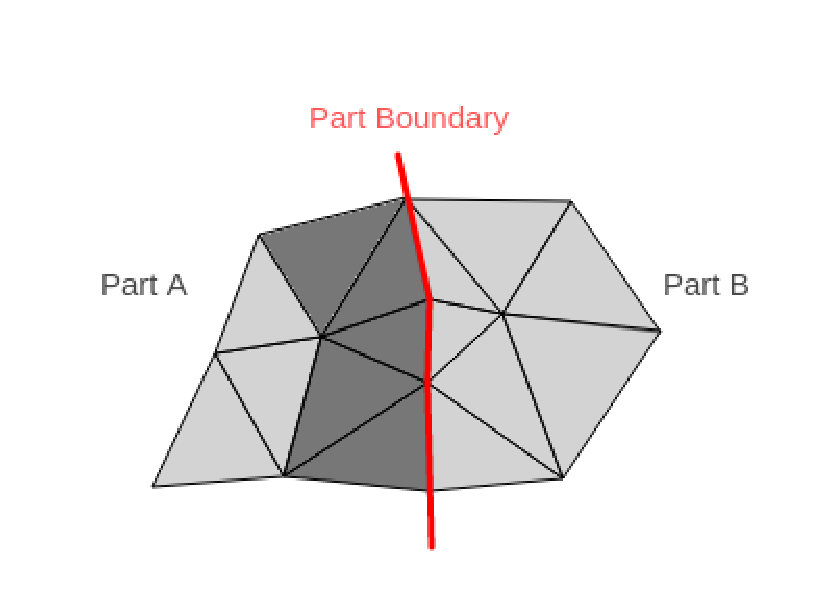
\includegraphics[width=0.8\textwidth]{ghost.eps} 
\caption{\label{fig:ghost3} A layer of ghosted elements from part A to part B. The darker elements represent all the elements on part A that part B will copy to create its remote mesh.}
\end{figure}

Given a
uniformly-weighted mesh we first partition it one part to $N$ parts using
Zoltan's interface to ParMETIS's multi-level graph-based method.
Once distributed we then run ghost-aware diffusive load balancing using
ParMA~\cite{SmithParma2015} to get a final mesh that is well balanced for
analysis procedures.
ParMA's partition improvement procedures account for
the ghosted layers using a combination of existing element selection criteria
and an extended `weight' tracking mechanism.
The weight tracking extension relies on the exact knowledge of the change to the
ghosted elements as elements on a heavy part are selected for migration to a
light part.
ParMA also balances degree-of-freedom holders defined by 
hierarchical Nedelec basis functions CITE 2009 OMEGA3P PAPER ~\cite{ingelstrom2006new}.
CWS - DESCRIBE THE PHASES OF PARMA
For first order elements this requires balancing edges.
Second order elements requires edges and faces, and above that edges, faces, and
regions need to be balanced.
We have implemented ParMA ghost-aware edge balancing.

\section{Status}\label{sec:software}
Omega3P currently supports reading a curved mesh from a NetCDF formatted file
into a DistMesh, or reading a PUMI mesh directly.
If a serial DistMesh was read it is converted to a PUMI-APF mesh and then 
partitioned using ParMETIS via the Zoltan interface.
Prior to running the Omega3P analysis the partition is balanced using ParMA
iterative diffusion methods.
ParMA diffusion directly modifies the distribution of the PUMI-APF mesh to
balance the degree of freedom holders and the ghosted mesh entities.
Lastly, prior to running the analysis, the PUMI-APF mesh is converted to
DistMesh.

CWS - SAY WHAT THE PROBLEMS WERE AND WHAT WE DID TO FIX THEM
\begin{itemize}
  \item repo contained large input and output data files - split data files into separate tarball
  \item configuration file on cori and edison used combination of preinstalled
    libraries and specific !modified! versions of libraries - we documented the
    exact changes needed and avoided use of system installs when possible
  \item did not support latest version of parmetis and zoltan - APIs updated 
  \item we built on the scorec workstations - demonstrated portability improvements
\end{itemize}

PUMI integration within Omega3p required understanding the Omega3P build process
and software dependencies so we could build and test on the SCOREC workstations
and the NERSC Cray systems (Cori Phase I and Edison).
The dependencies and the build process is now documented and Boost-Build
configuration files updated to use the latest system compilers.
The only dependency conflict we encountered stemmed from Omega3P's use of old
Zoltan and ParMETIS versions; PUMI requires the latest versions which have
slightly different APIs.
So, we ported the Omega3P API calls to use the Zoltan (3.81) and
(Par)METIS (4.0.3) APIs and modified the build system accordingly.
To ensure these changes and the other build system modifications did not break
Omega3P we also scripted execution of regression tests.

\section{Results and Next Steps}\label{sec:results}

CWS - REVISE
We ran Omega3P and Omega3P+PUMI on the \textit{cav17} model with a 318118
element quadratic mesh on up to 128 cores (32 cores per node) of the NERSC Cori
Phase I system.
The runtime of Omega3P+PUMI and Omega3P is shown in Figure~\ref{fig:time}.
Analysis of timing results is ongoing to determine where we are saving and
losing time.
Peak memory usage across all processors is shown in
Figure~\ref{fig:memusage}.
As expected, the Omega3P+PUMI memory usage is higher than Omega3P.
At 64 cores there is a 2\% increase and at 128 cores there is an 8\% increase.
Figures~\ref{fig:vtx} and~\ref{fig:elm} respectively show the total count
(ghost+owned) and ghost + owned imbalance of vertices and
elements.
We suspect that the increased number of entities will account for some portion
of the runtime and memory usage increases with core count, but a more detailed
comparison of the imbalance and memory usage is required.

\begin{figure}[ht]
\centering
  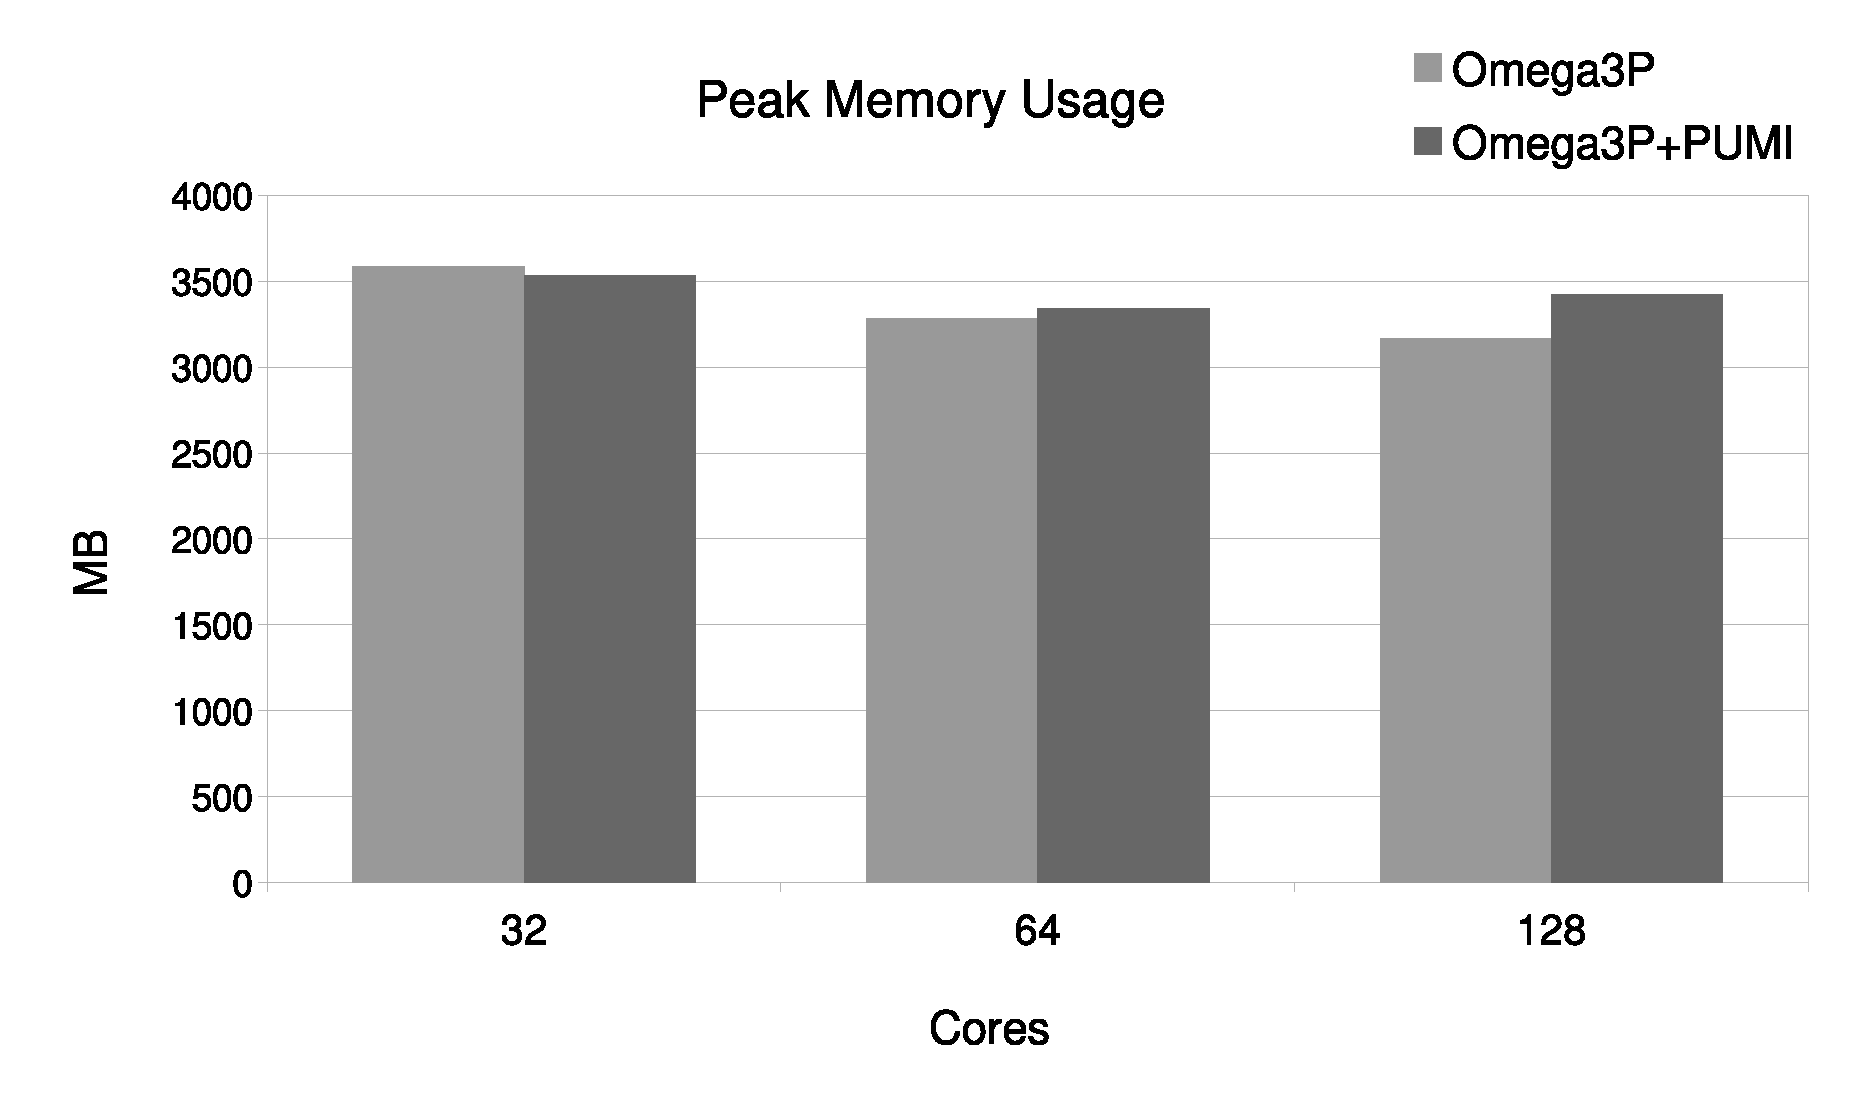
\includegraphics[width=\textwidth]{peak-memory-usage.eps}
  \caption{\label{fig:memusage} Peak memory usage.}
\end{figure}

\begin{figure}[ht]
\centering
  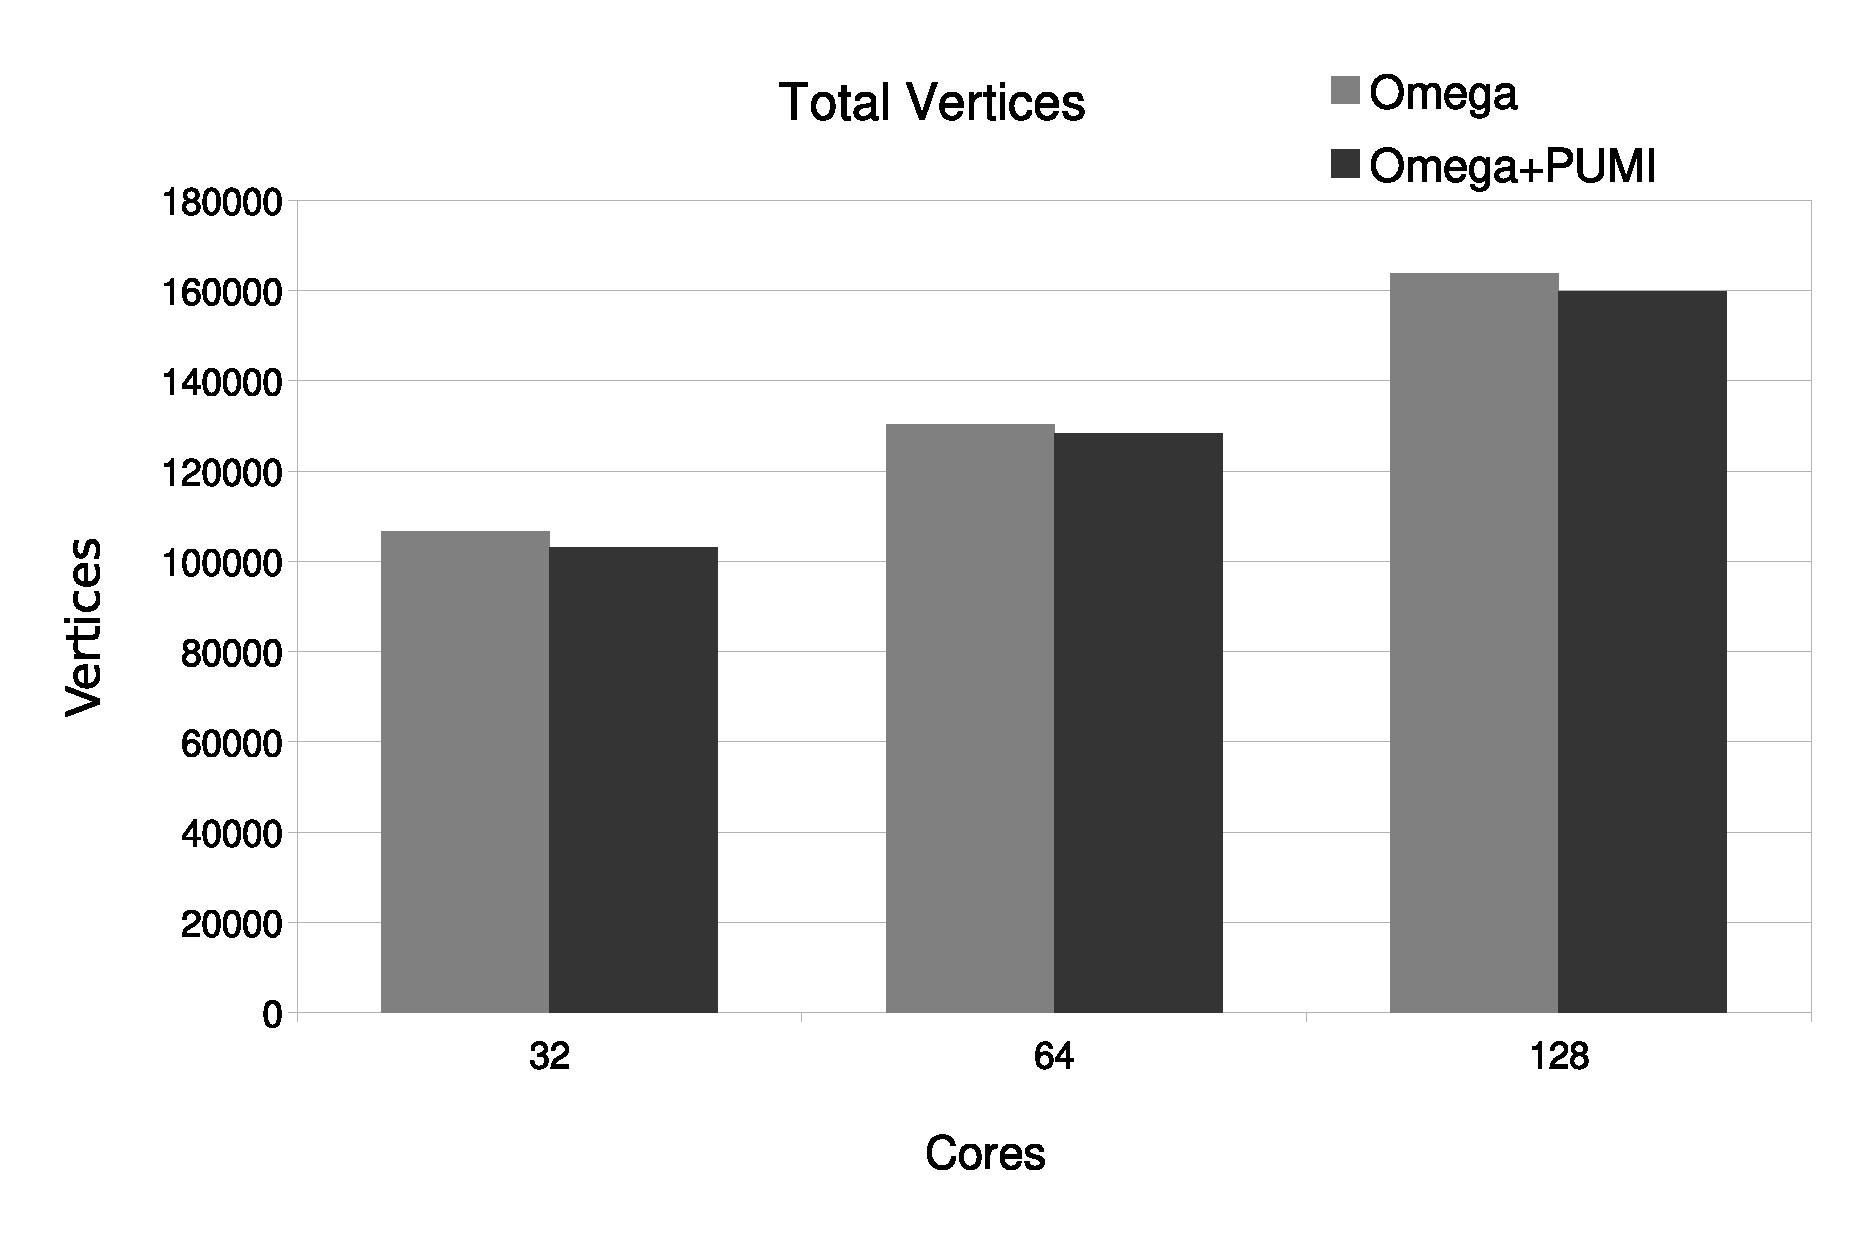
\includegraphics[width=\textwidth]{total-vtx.eps} \\
  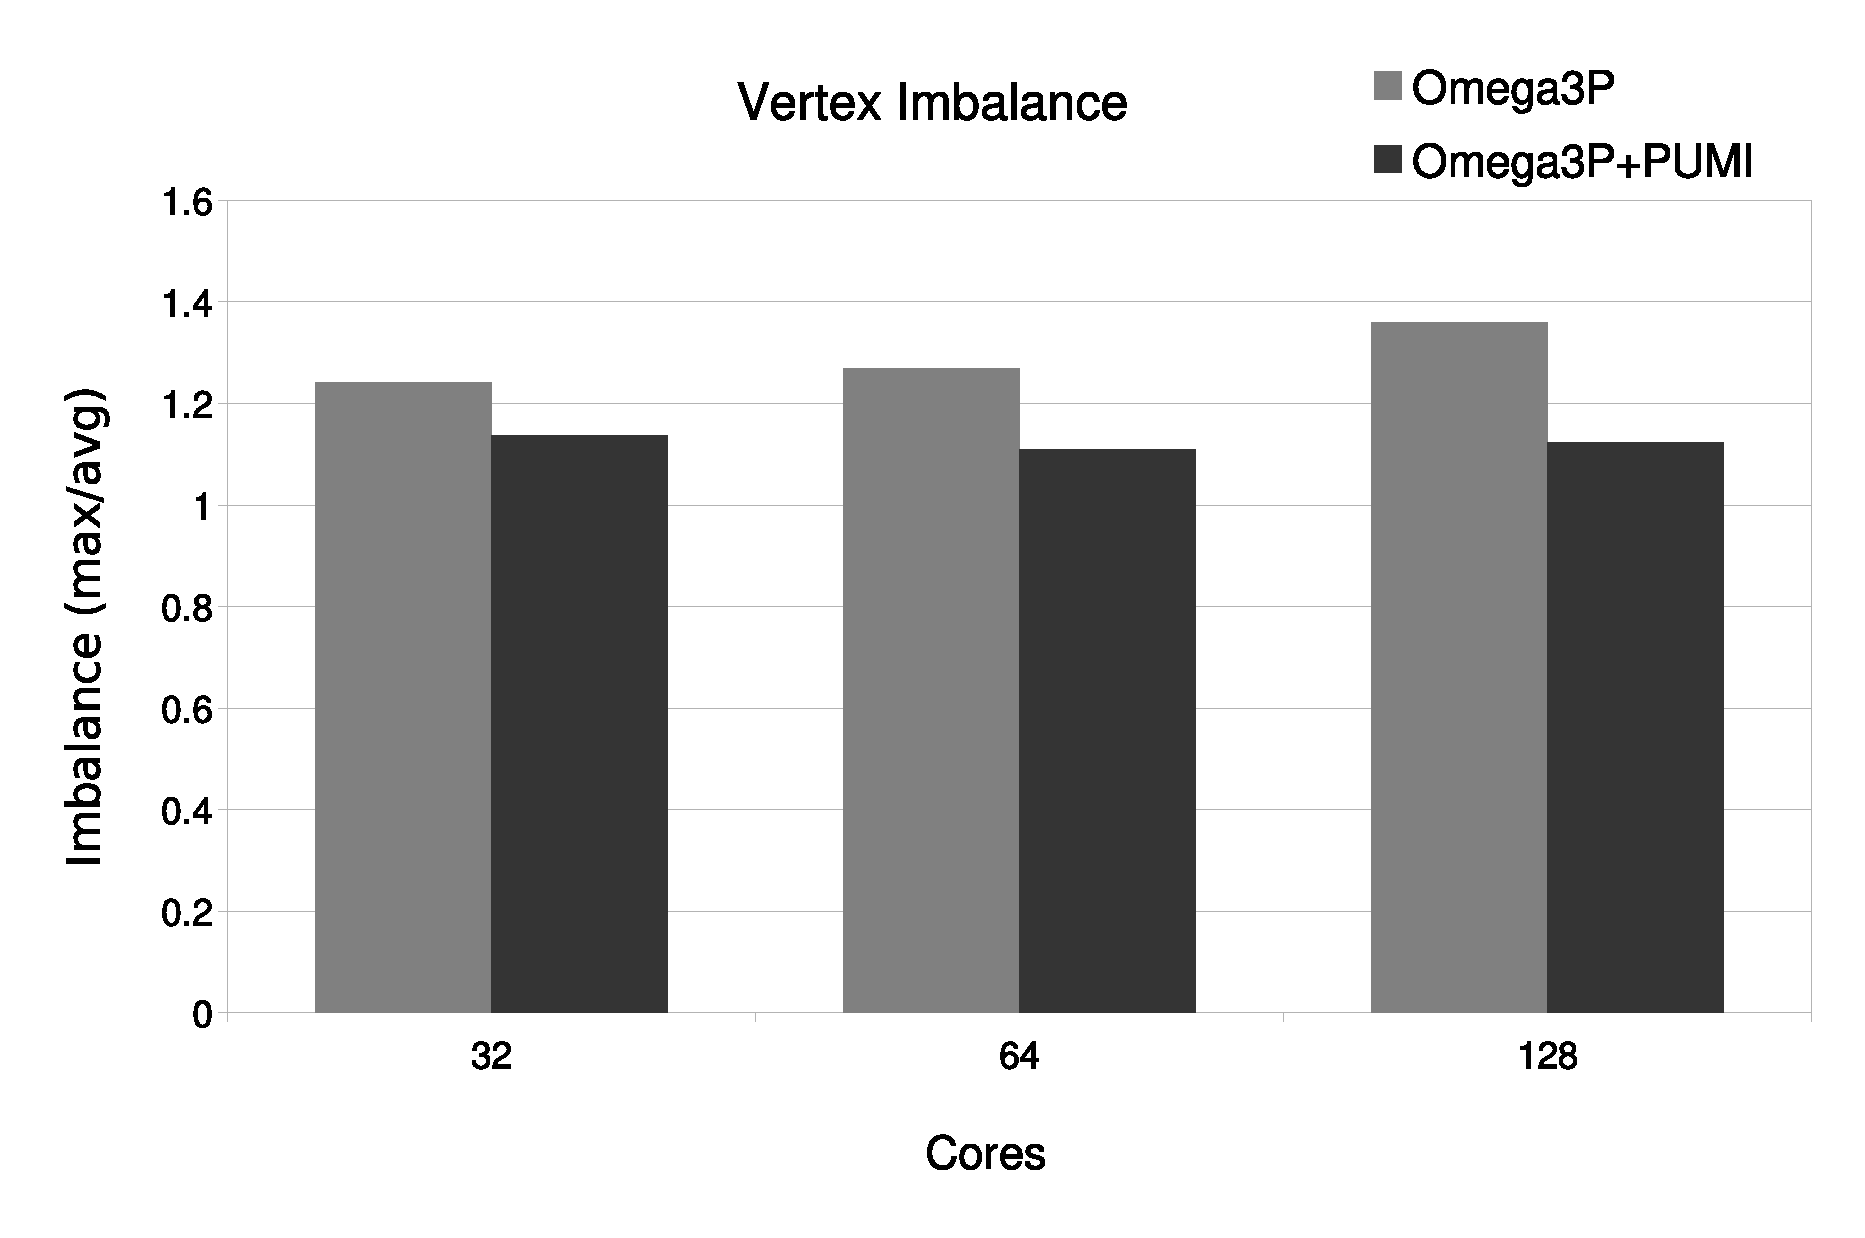
\includegraphics[width=\textwidth]{vtx-imb.eps} \\
  \caption{\label{fig:vtx} Total (ghost+owned) vertex count and vertex imbalance.}
\end{figure}

\begin{figure}[ht]
\centering
  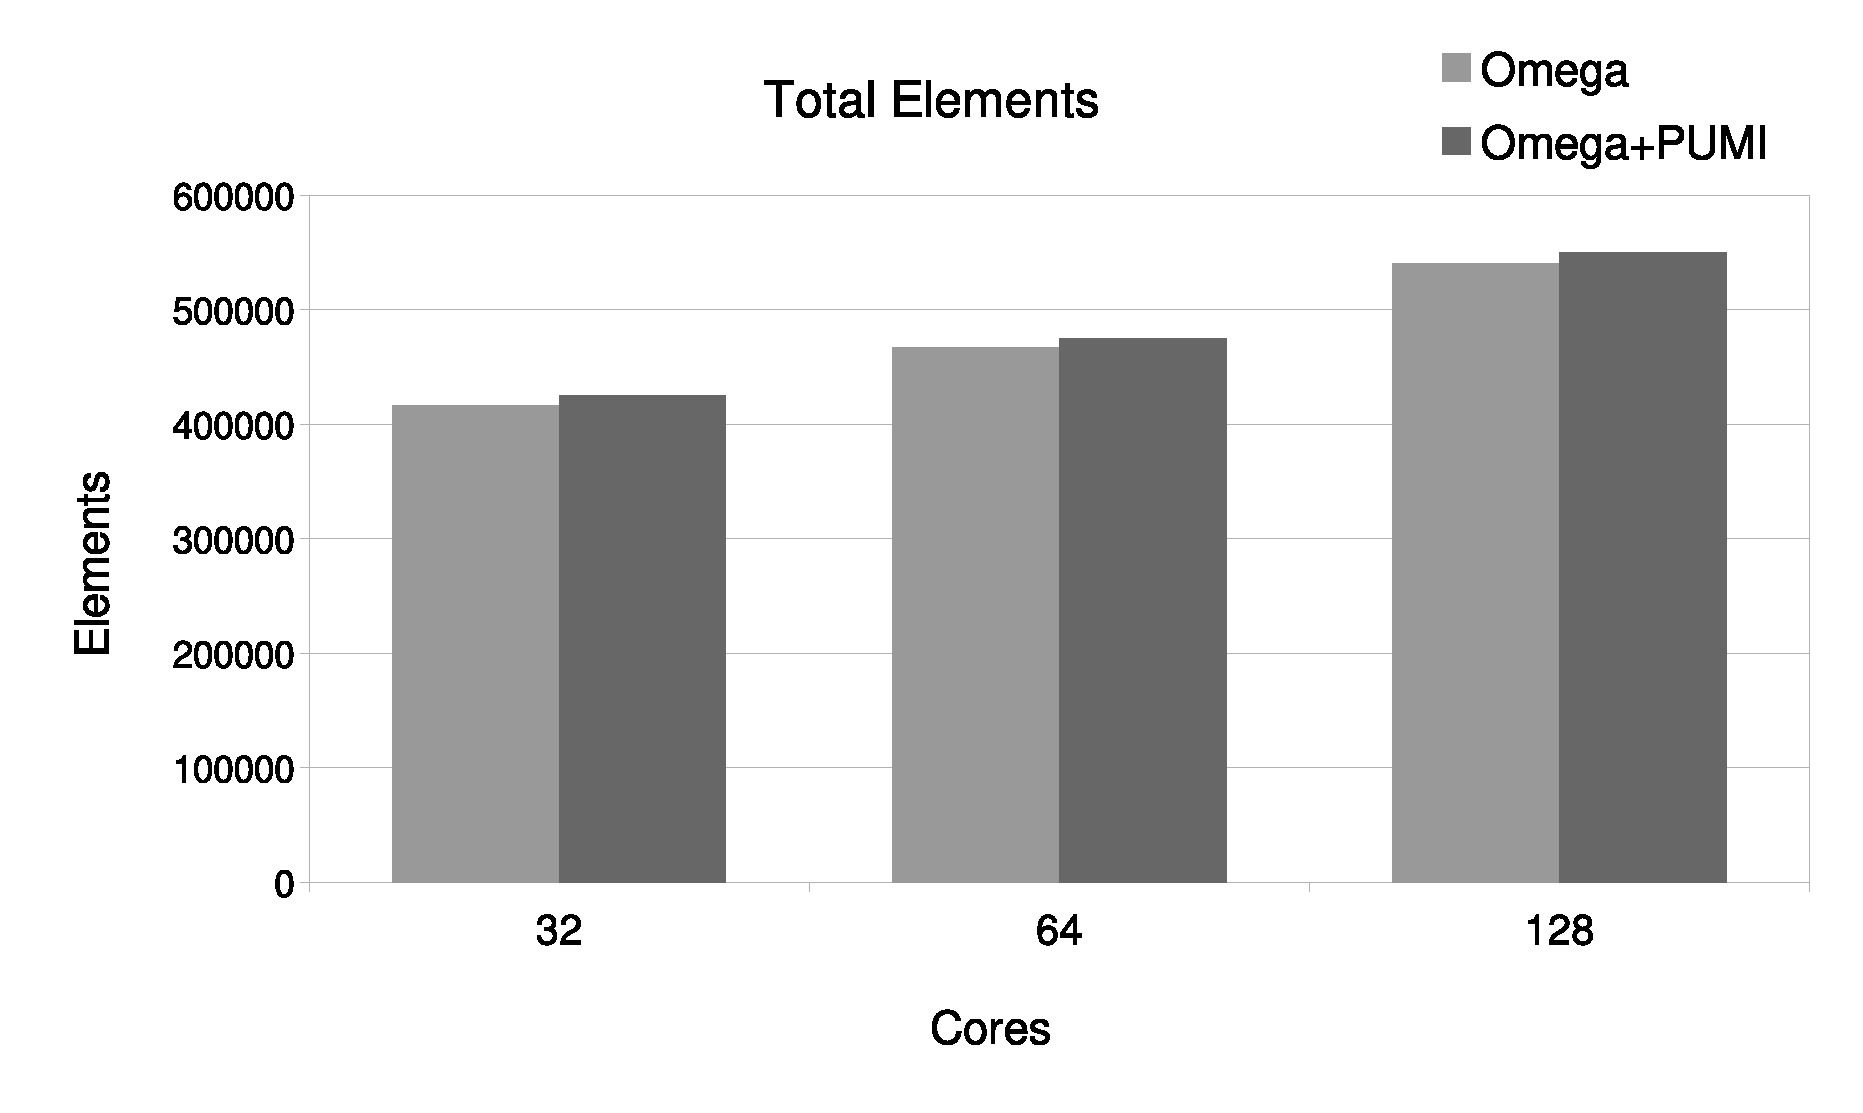
\includegraphics[width=\textwidth]{total-elms.eps} \\
  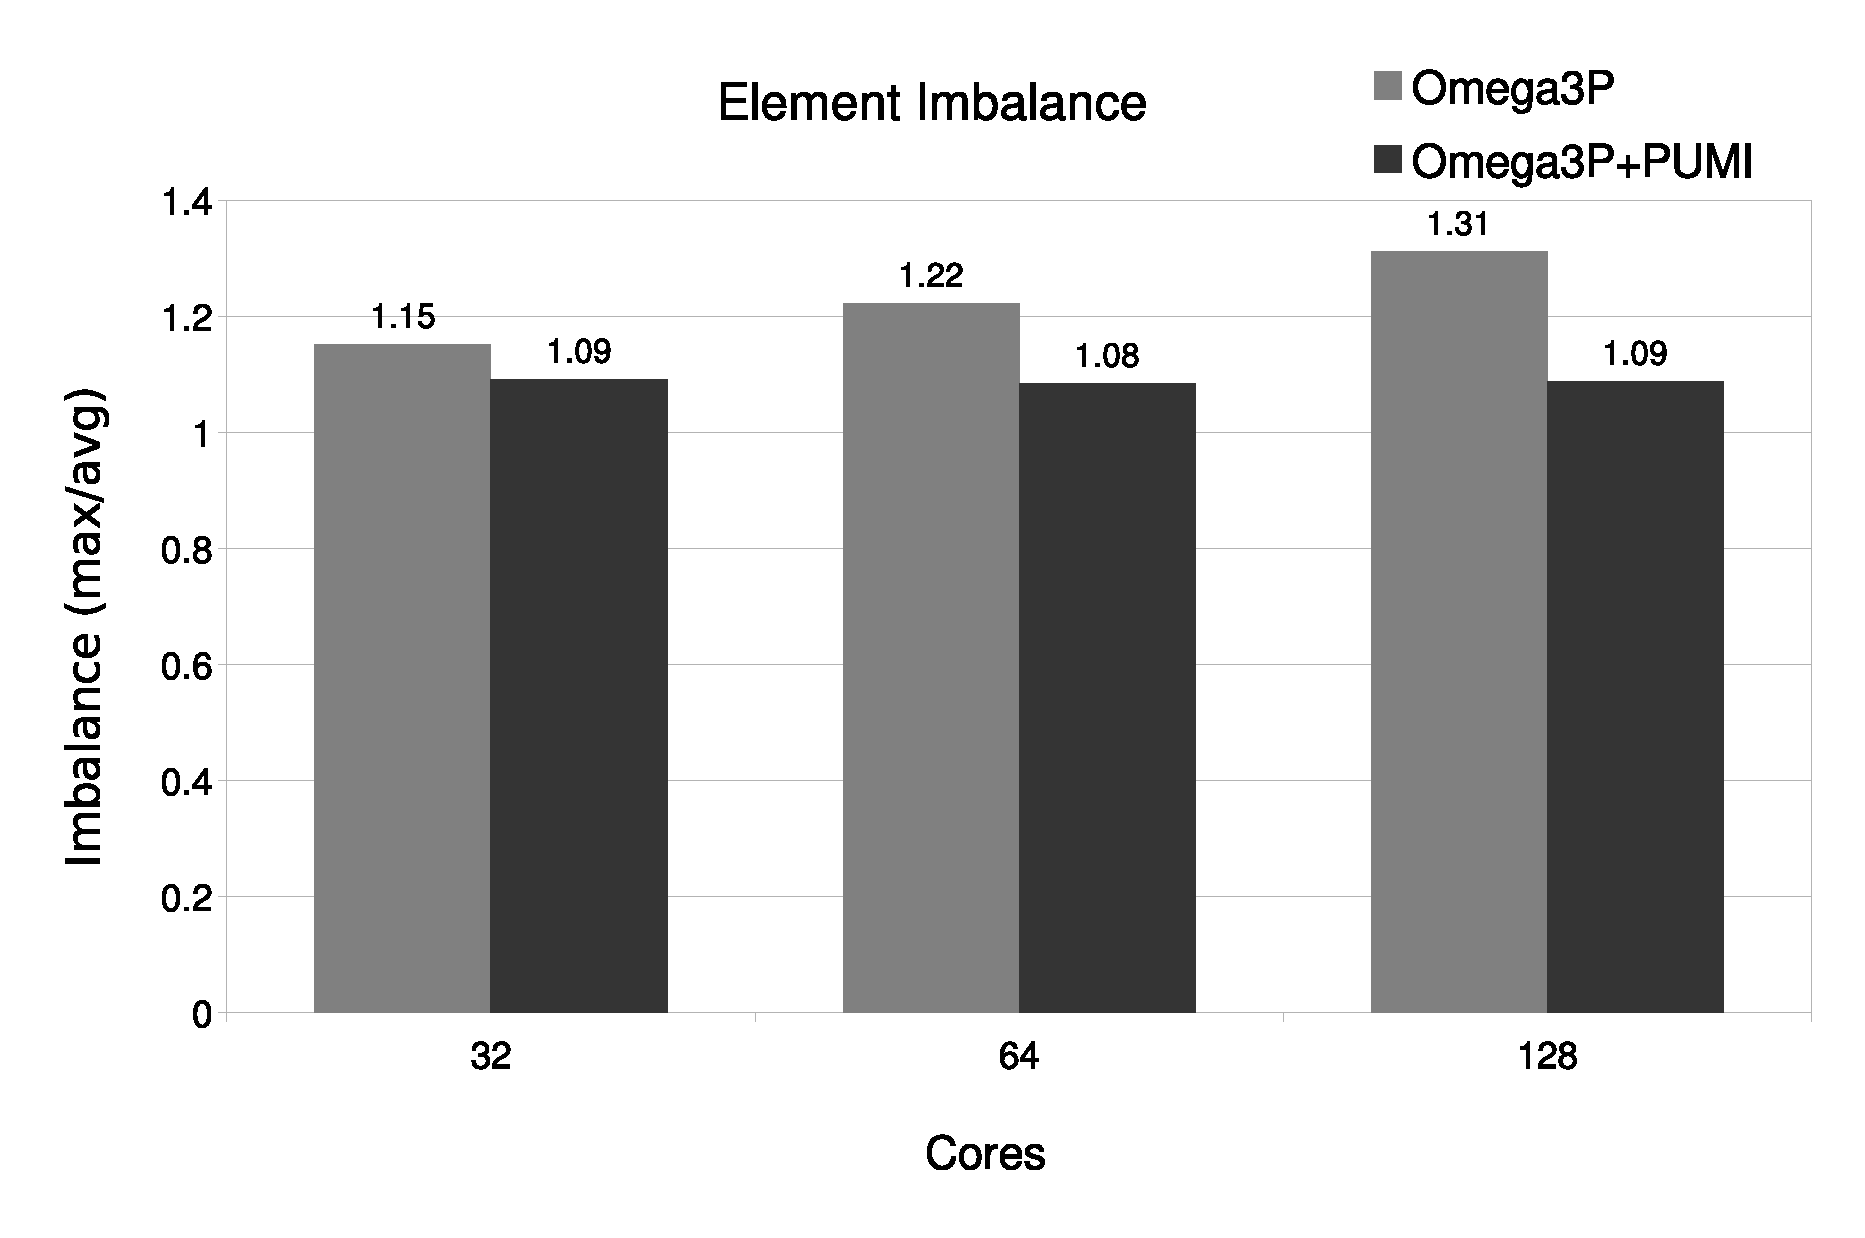
\includegraphics[width=\textwidth]{elm-imb.eps} \\
  \caption{\label{fig:elm} Total (ghost+owned) element count and element imbalance.}
\end{figure}

Our next step will be to perform a detailed analysis of the runtime and memory
usage.
Assuming the increased entity count has a is a significant issue, we will then modify
the ParMA ghost balancer as described in Section~\ref{sec:parma}.
After we have shown runtime improvements we plan to automate our regression
tests and work with SLAC developers to merge our changes into
the ACE3P central repository and make our documentation accessible.

\newpage \bibliographystyle{plain}
\bibliography{scorec-refs/partition,scorec-refs/meshdb,scorec-refs/hardware,scorec-refs/io,scorec-refs/frameworks,scorec-refs/cr,scorec-refs/fem}

\end{document}


